%%%%%%%%%%%%%%%%%%%%%%%%%%%%%%%%%%%%%%%%%%%%%%%%%%%%%%%%%%%%
%%% ELIFE ARTICLE TEMPLATE
%%%%%%%%%%%%%%%%%%%%%%%%%%%%%%%%%%%%%%%%%%%%%%%%%%%%%%%%%%%%
%%% PREAMBLE 
\documentclass[9pt,lineno]{elife}
% Use the onehalfspacing option for 1.5 line spacing
% Use the doublespacing option for 2.0 line spacing
% Please note that these options may affect formatting.

\usepackage{lipsum} % Required to insert dummy text
\usepackage[version=4]{mhchem}
\usepackage{siunitx}
\DeclareSIUnit\Molar{M}
\usepackage{indentfirst} %I prefer to have indents following section headings, I find it to be more consistent in style throughout document

%%%%%%%%%%%%%%%%%%%%%%%%%%%%%%%%%%%%%%%%%%%%%%%%%%%%%%%%%%%%
%%% ARTICLE SETUP
%%%%%%%%%%%%%%%%%%%%%%%%%%%%%%%%%%%%%%%%%%%%%%%%%%%%%%%%%%%%
\title{Transcriptional dynamics of influenza virus infection in single cells}

\author[1]{Alistair B. Russell}
\author[2]{Cole Trapnell}
\author[1,2*]{Jesse D. Bloom}
\affil[1]{Basic Sciences Division and Computational Biology Program, Fred Hutchinson Cancer Research Center, Seattle, United States}
\affil[2]{Department of Genome Sciences, University of Washington, Seattle, United States}
\corr{jbloom@fredhutch.org}{}

% \presentadd[\authfn{5}]{eLife Sciences editorial Office, eLife Sciences, Cambridge, United Kingdom}

%%%%%%%%%%%%%%%%%%%%%%%%%%%%%%%%%%%%%%%%%%%%%%%%%%%%%%%%%%%%
%%% ARTICLE START
%%%%%%%%%%%%%%%%%%%%%%%%%%%%%%%%%%%%%%%%%%%%%%%%%%%%%%%%%%%%

\begin{document}

\maketitle

\begin{abstract}
Influenza virus infection induces large changes in cellular transcription.
Previously this has mostly been looked at using bulk measurements
Here we examine the process at the level of single cells.
We find extremely wide variation in the extent of viral gene transcription across infected cells.
IFN induction is very rare.
Some cellular pathways may be consistently altered in cells with high burden of viral transcripts.
Overall, highlights remarkable heterogeneity in the outcome of infection.
\end{abstract}


\section{Introduction}

Heterogeneity is important in a lot of cellular processes even when isogenic~\citep{shalek2013single,shalek2014single}.

Population (genetic) heterogeneity is also important. 
Viral quasispecies, cancer single-cell, etc.
Salmonella paper (PhoP).

Literature on viral burst-size heterogeneity.
This goes back to Delbruck, Andino polio paper~\citep{schulte2014single}, the MDCK / flu paper.

Discuss segmented nature of influenza.
Maybe in the context of how this could further increase heterogeneity because there is a lot of potential for entire genes to be missing.
Includes Yewdell and Lowen papers.

\section{Results}

\subsection{Strategy to measure mRNA transcription in single infected cells.}
% \subsection{Initial Steps to Generate Robust Single-Cell Kinetic Observations}
We chose to perform single-cell mRNA sequencing using a droplet-based system that physically isolates single cells prior to performing reverse-transcription.
Each droplet contains a unique \emph{cell barcode} that is used to tag all mRNAs from that cell during reverse-transcription.
a random \emph{unique molecular identifier (UMI)} is additionally appended to each mRNA molecule during reverse transcription.
Sequencing of the 3' ends of the mRNAs therefore enables quantification of the number of different molecules of each mRNA species that are captured per cell.

While infected cells will express viral as well as cellular mRNAs, the cell barcodes and UMIs do not enable direct detection of whether a cell was initially infected by one or multiple viral particles.
We therefore engineered an influenza virus that additionally carried \emph{viral barcodes} near the 3' end of each transcript (Figure~\ref{fig:workflow}A).
These viral barcodes consisted of two synonymous mutations designed to fall in the 3' portion of the mRNAs sequenced by our approach.
Critically, these mutations did not appear to dramatically impact viral growth kinetics. (Figure~\ref{fig:workflow}B).
We then infected A549 human lung carcinoma cells with an equal mix of the wildtype and synonymously barcoded viruses.
Cells infected by a single virion should exclusively express mRNAs from either wild-type or synonymously barcoded virus, while cells that are co-infected with multiple virions will frequently express mRNAs from both the wildtype and synonymously barcoded viruses (Figure~\ref{fig:workflow}C).
\begin{figure}
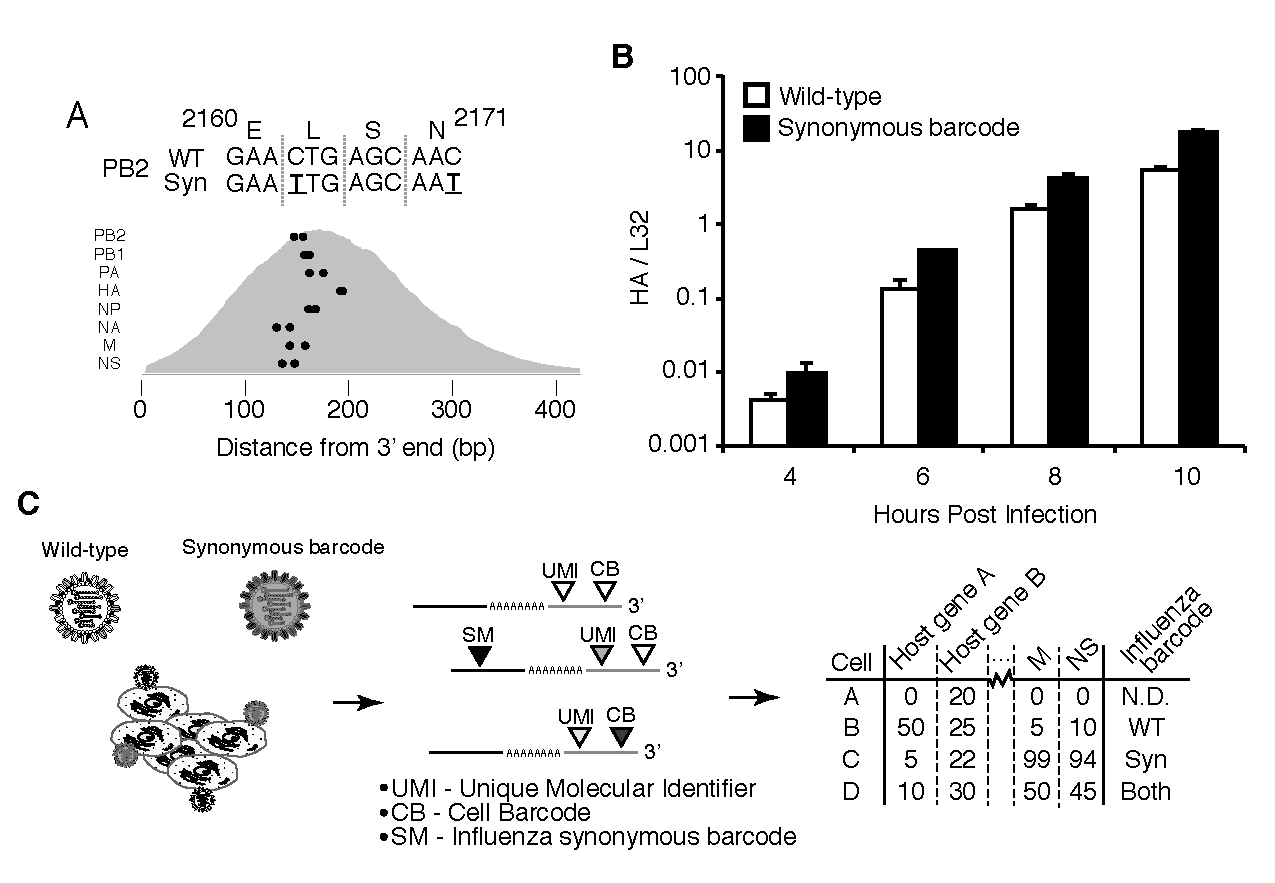
\includegraphics[width=0.8\linewidth]{figures/Workflow/workflow.pdf}
\caption{\label{fig:workflow}
{\bf (A)}  Design of synonymously barcoded virus. Top, comparison of wild-type and mutant PB2 sequences, with nucleotide positions (as measured in mRNA) and amino acid identities. Bottom, locations of two mutations comprising synonymous viral barcode mapped on top of read depth of the \emph{FTL} locus in uninfected A549 cells.
{\bf (B)} Growth kinetics are conserved between wild-type and synonymously barcoded virus. qPCR measurements of HA mRNA at the indicted time points normalized to the housekeeping control, \emph{L32}.
{\bf (C)}  Schematic of workflow. A549 cells were infected with an equal mixture of mutant and wild-type virus. Using a reverse-phase emulsion, cells are physically separated and cDNA libraries are generated containing the indicated barcodes. Subsequent amplification and sequencing of libraries permits the identification and assignation of transcript abundances to individual cells. Additional information from our influenza synonymous barcode allows for the generation of categorical data with respect to infection state. Abbreviations WT: wild-type, Syn: Synonymous Barcode.
}
\figdata{Sequences of wildtype and synonymously barcoded viruses are in FASTA file XXX (add this FASTA file to the figures directory).}
\end{figure}

We also took great care to produce stocks of virus that we expected to be relatively ``pure.''
Many viruses, including influenza, rapidly diversify into an array of biologically active viral particles, many of which can have mutations or deletions in essential viral genes.
For influenza virus, one abundant forms of these defective particles arises from deletions that occur in the three viral segments encoding the tripartite viral polymerase.
These defective particles become particularly abundant when the virus is grown at high multiplicities of infection, where virions with defective genes can be complemented by co-infection with other virions.
To keep the level of these defective particles as low as possible, we propagated our viral populations at low multiplicity of infection.
We then validated that compared to virus propagated at high multiplicity of infections, our viral populations exhibited a much greater purity of infectious particles.
We validated this by assessing the ratio of infectious particles to viral-RNA molecules (Figure~\ref{fig:viruspopulations}A) and to particles that induce cellular expression of a single viral protein (Figure~\ref{fig:viruspopulations}B).
We also showed that our viral populations induced much less interferon than a population propagated at higher multiplicity of infection as expected because...
Lastly, our populations induced far less interferon than a high defective control, consistent with prior observations that such stocks are more immunostimulatory (Figure~\ref{fig:viruspopulations}D).

\begin{figure}
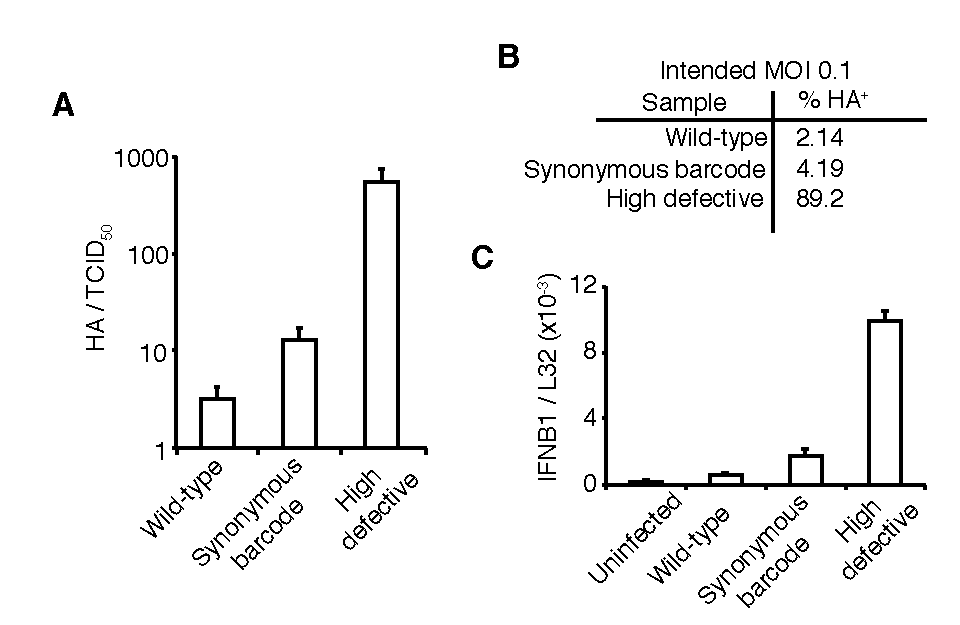
\includegraphics[width=0.7\linewidth]{figures/Validating_barcode_virus/validating_populations_D02.pdf}
\caption{\label{fig:viruspopulations}
Panel A has now moved to the other figure.
In panel A, the vertical alignment is a bit off for a few of the tick labels.
Space between ``HA'' and ``TCID50'' on the y-axis.}
\end{figure}

\subsection{Population-Level Measurements Validate Dataset.}
Using these validated populations, we tracked growth kinetics in our target cell line at an infectious dose targeting a final infection rate of 5 percent as determined by flow cytometry. 
We observed rapid transcript accumulation through 10 hours, which then tapered off --- potentially representing new rounds of infection rather than progression in initially infected cells (supplemental figure). 
We then chose three time points (6,8, and 10h) reflecting dramatically different influenza burden (and thus different stages in influenza replication) for this study.

\begin{figure}
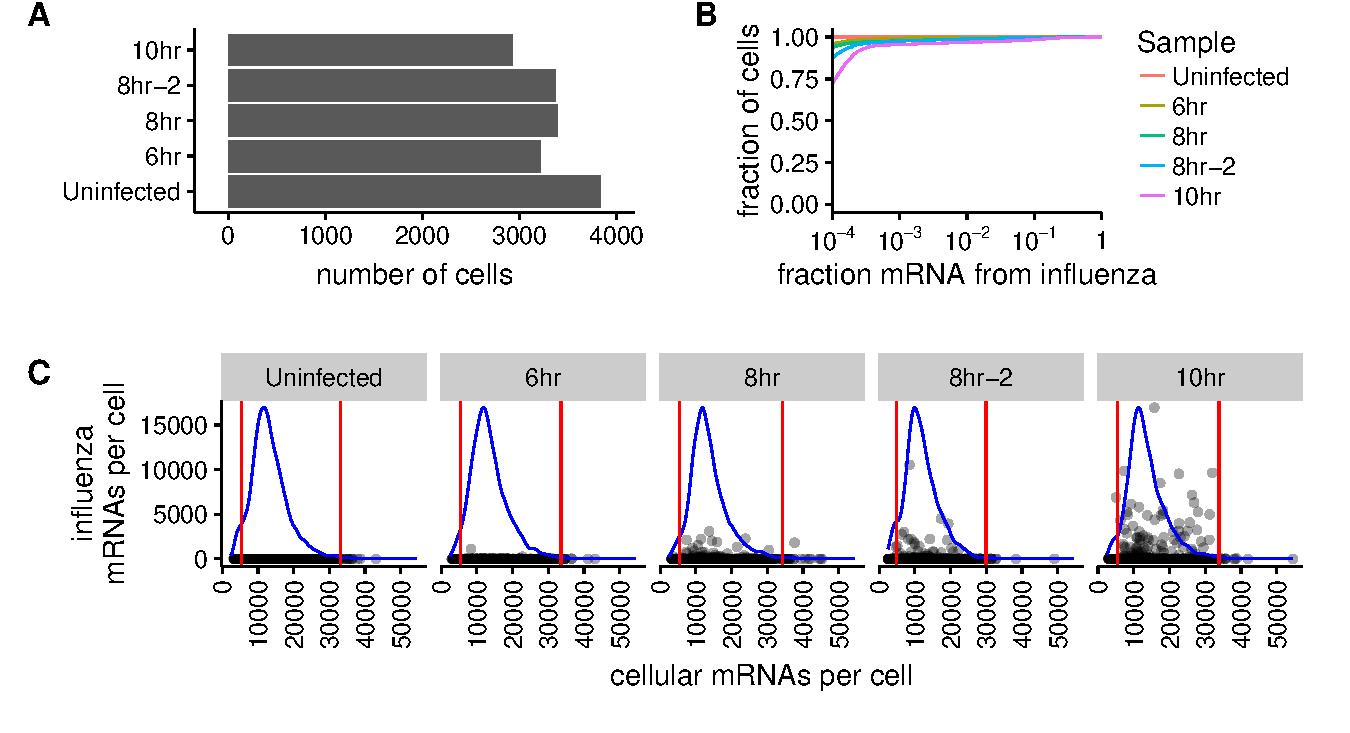
\includegraphics[width=\linewidth]{figures/p_cell_mRNA_summary.pdf}
\caption{\label{fig:cells}
Overview of amounts of cellular and influenza virus mRNAs detected in each cell.
{\bf (A)} 
Number of cells captured for each sample.
{\bf (B)} 
Cumulative fraction plot showing the amount of mRNA derived from influenza for each sample.
In all samples, most cells had little or no influenza mRNA.
{\bf (C)} 
The number of cellular and viral mRNAs for each cell is plotted as a point.
The blue lines show the overall distribution of the number of cellular mRNAs per sample.
Cells that fell outside the red lines were removed as outliers.
At later timepoints, a small number of cells had a very high number of viral mRNAs.
}
\end{figure}

Before proceeding with more detailed analyses, we first examined population-level data to confirm the validity of our approach. 
We not only generated data for our three time points and a matched uninfected control, but also performed a biological replicate at 8 hours to determine whether our findings could be dominated by inter-sample or technical variation rather than biological processes driven by influenza. 
We sampled roughly equivalent number of cells per time point at an equivalent sequencing depth per cell - granting similar probability to observe rare events across datasets (Figure~\ref{fig:cells}A) (ADD SUPPLEMENTAL OF DEPTH/CELL?). 
Overall we observed highly similar distributions of transcript abundance between samples (Figure~\ref{fig:cells}B). 
This suggests that, in a rough global sense, transcriptome dynamics are relatively unperturbed and that influenza, if it is driving dramatic changes in transcript abundance and/or growth state, must be doing so in only a small subset of cells. 
More importantly, with the confidence that the average cellular state is similar between time points, we can better regard changes in subpopulations between time points as bone-fide progression in influenza replication rather than inter-sample variation.

In addition to analyses regarding global transcript abundance, we were also able to successfully detect increasing numbers of influenza transcripts as our experiment progressed (Figure~\ref{fig:cells}C). 
Moreover, there appeared to be only a few cells at each time point making considerable contributions to the influenza transcript pool, consistent with our desired low level of infection. 
With these metrics, we felt confident proceeding to more detailed analyses of influenza replication kinetics and impact on these populations.

\subsection{Synonymous Barcodes Provide An Empirical Means of Setting Infection Thresholds.}
As a first step in understanding influenza replication at a single-cell level, we must derive a threshold for identifying infected cells. 
Crucial to our experimental design, we were able to detect both wild-type and synonymous influenza variants at all three timepoints in all eight segments, at levels permitting identification of cells infected with one, or both strains (Figure~\ref{fig:viralbarcodes}-Figure~supplement~\ref{figsupp:barcodescalled}). 
This was true of about half of the transcripts surveyed, matching the read-density of our preliminary experiments. 
These barcodes partitioned non-randomly between cells, as expected if derived from single infectious events (Figure~\ref{fig:viralbarcodes}A,B). 
This grants us the power to develop an empirical threshold for calling influenza-infected cells versus those that might have reads derived from lysis of infected cells. 
Reads derived from lysed cells should exhibit random partitioning ? sampling each barcode according to its overall abundance in the experiment. 
Therefore, when ordering all cells at all timepoints according to the number of influenza reads observed and the relative abundance of each barcode, we can set our detection threshold as the point at which barcodes reliably exhibit non-random partitioning - that is when all segments in a given cell are frequently derived from either our synonymous or wild-type virus but not both (Figure~\ref{fig:viralbarcodes}C). 
Notably, this strategy relies heavily on a relatively low MOI, as high rates of coinfection would stymie this approach (Figure~\ref{fig:viralbarcodes}D,E) . 

Few coinfections

Setting threshold: Assumes rare barcode events are due to lysis (or misannotation)  and that two values SHOULD correlate
Validating evidence/assumption two values correlate - flow data, flow diagram and quantile-normalized data. Include replicates in supplement.

Once defined, we have some statistics.

Presumably this subsection basically covers \ref{fig:viralbarcodes}. 

\begin{figure}
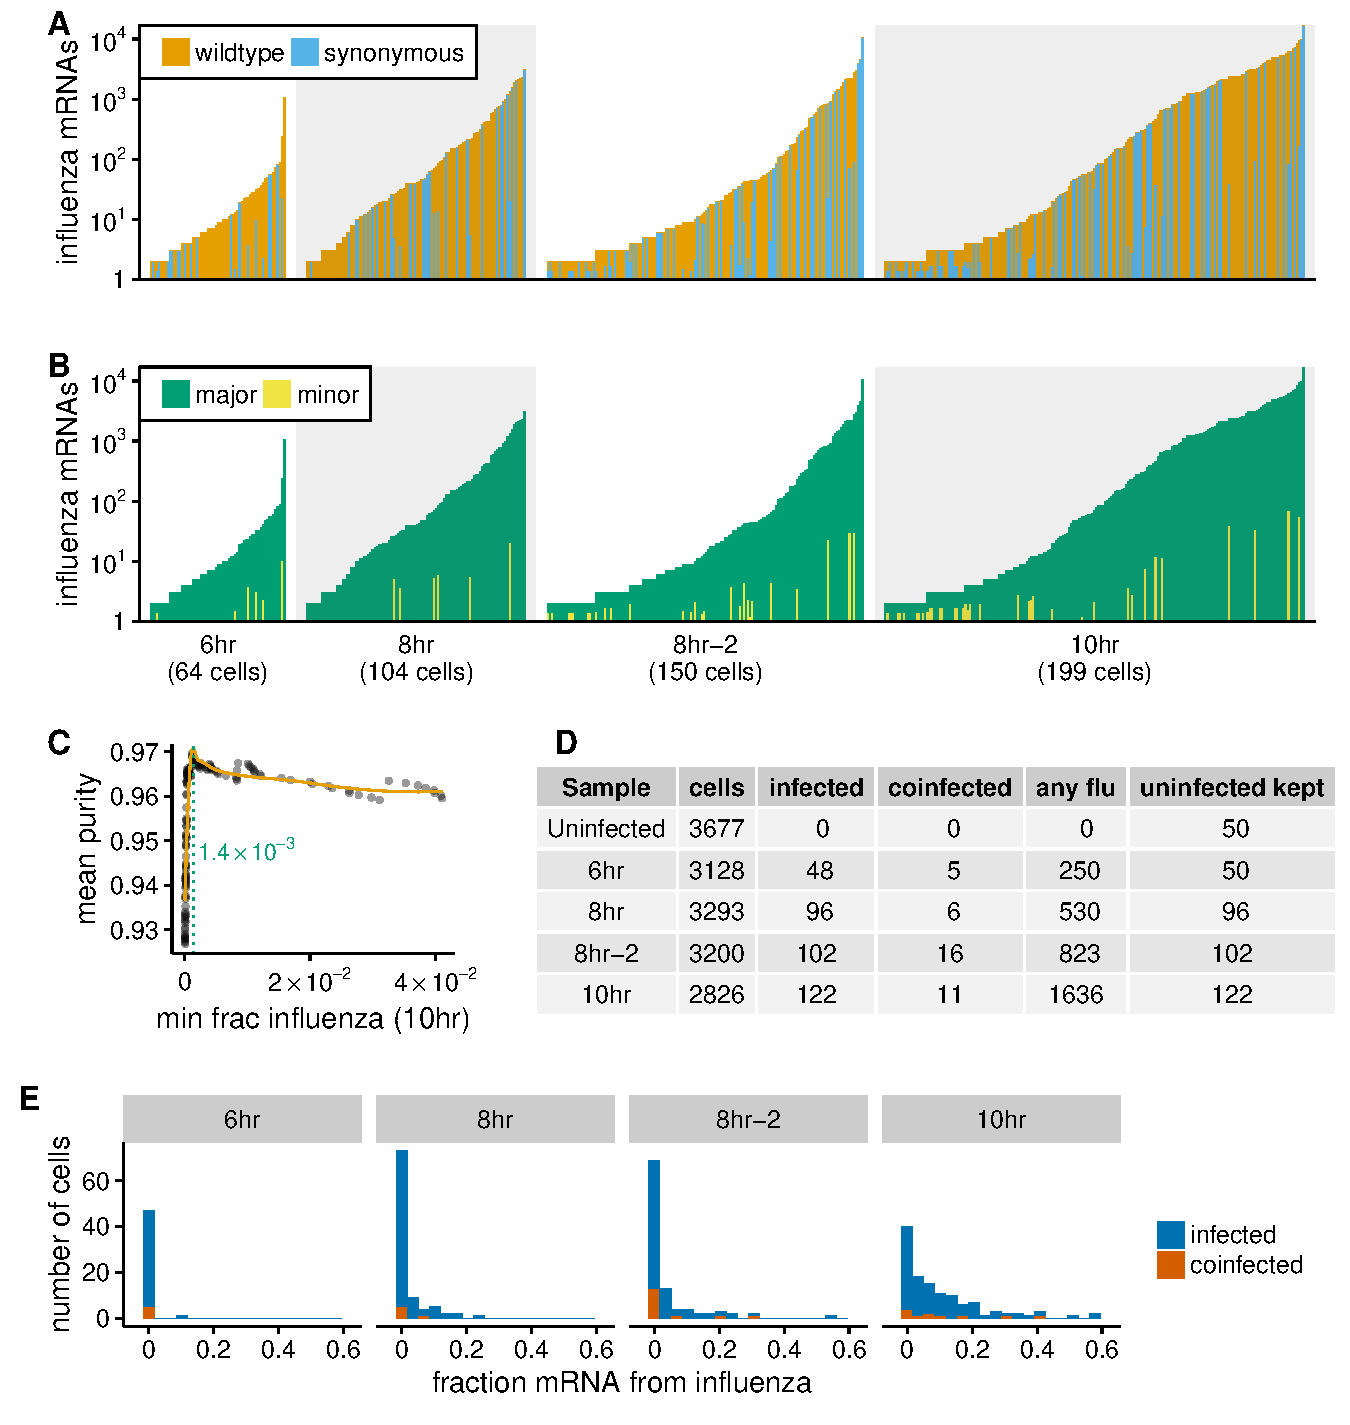
\includegraphics[width=\linewidth]{figures/p_frac_flu_summary.pdf}
\caption{\label{fig:viralbarcodes}
Synonymous barcodes near the 3' end of the influenza virus mRNAs were used to identify co-infection and distinguish true infections from cells that contained a few spurious viral reads.
{\bf (A)}
For all cells with at least two viral mRNAs for which the synonymous barcode could be called, each line is proportional to the logarithm of the number of viral mRNAs in that cell.
The bars are colored in linear proportion to the fraction of the viral mRNAs derived from either wildtype or synonymously barcoded virus.
{\bf (B)}
Same as (A), but now each bar is colored according to the relative proportions of the more common (major) and less common (minor) barcoded virus variant.
At low levels of viral mRNA there is often a roughly equal mix of barcodes, since many of these cells have simply picked up environment mRNA which is about equally likely to derive from either virus.
But at higher levels of viral mRNA, truly infected cells are mostly one pure barcode except for a few cells that are truly co-infected.
{\bf (C)}
We determined a cutoff for calling ``true'' infections by fitting a curve to the mean barcode purity of all cells with greater than a given fraction of their mRNA derived from virus.
We called the cutoff at the point at which purity stops increasing with the fraction of viral mRNA.
{\bf (D)}
The number of cells identified as infected and co-infected for each sample.
For all samples, the vast majority of cells were not infected, so for subsequent analyses we subsampled to a number of uninfected cells that was the greater of 50 or the number of infected cells.
{\bf (E)} 
The distribution of the fraction of mRNA derived from virus for each sample for both infected and co-infected cells.
For all samples, there is a very wide distribution of the amount of viral mRNA.
}
\figsupp[Number of viral barcodes called.\label{figsupp:barcodescalled}]{
The number of viral barcodes called for each sample and influenza gene segment. 
Viral transcripts are classified as \emph{syn} if they mapped to a synonymously barcoded influenza transcript, \emph{wt} if they mapped to a wildtype influenza transcript, \emph{invalid} if multiple reads for the same UMI differed on the status of the viral barcode, and as \emph{uncalled} if none of the reads for that UMI overlapped the region of the viral transcript containing the viral barcode.
}{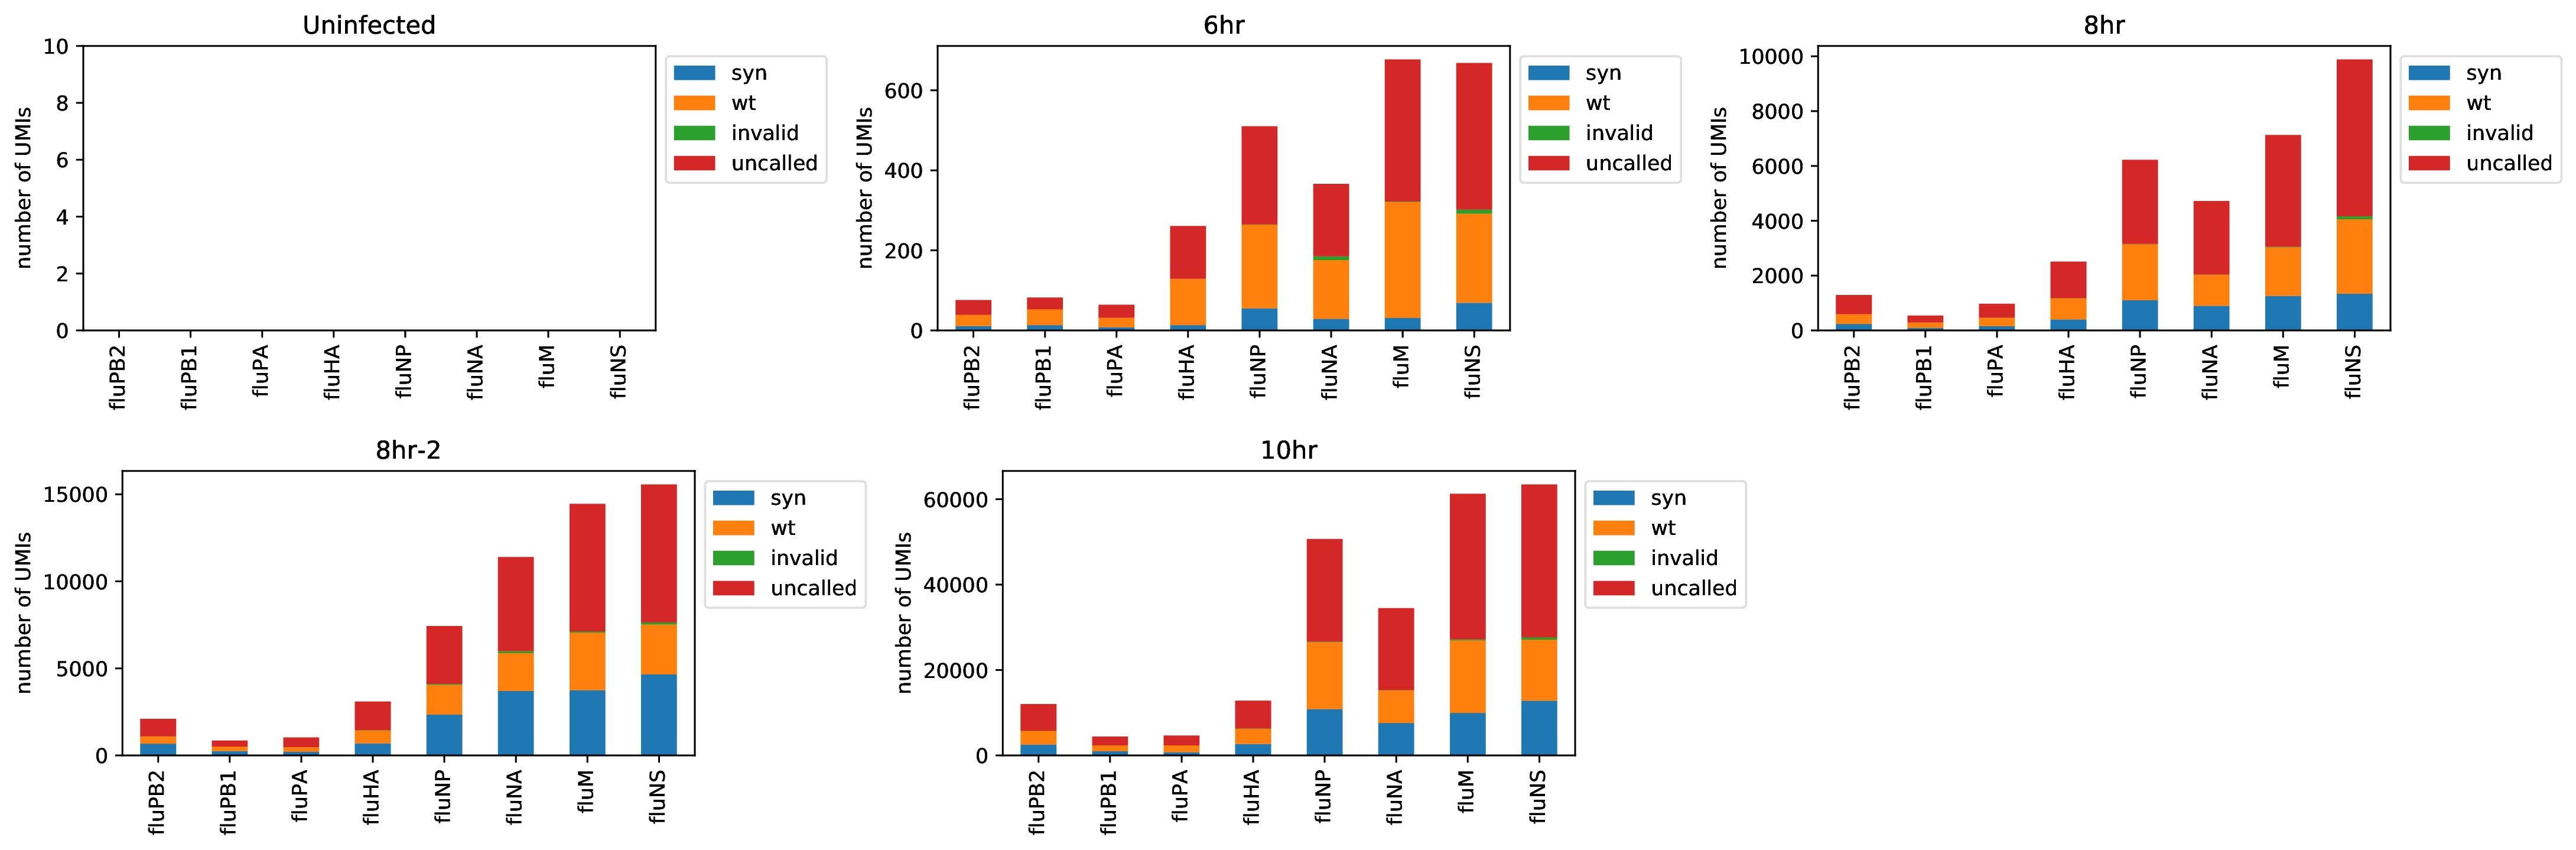
\includegraphics[width=\linewidth]{figures/synbarcodes_umistats.jpg}}
\end{figure}

\subsection{Influenza Exhibits A Broad Distribution of Productivity Partially Explained By Segment Absence.}
The absolute productivity of influenza infection as measured by the number of fully-infectious virions produced by a given cell is known to vary dramatically.  This observation is recapitulated in our data, wherein of the small portion of infected cells, a bare few contribute the majority of influenza transcripts (Figure~\ref{fig:cells}A) (MAYBE A MORE SPECIFIC SUPPLEMENTAL). As transcript abundance is highly dependent upon secondary transcript from de novo generated viral genomes, it can be presumed that when comparing between two cells, increased mRNA abundance is likely correlated with increased viral genome production, which in turn is highly predictive of viral productivity. It is thought that one driver of the observed variation in influenza productivity is the segmented nature of the influenza genome. Several groups have described that the majority of infections fail to express at least one of the eight influenza segments. Our datasets produce a similar pattern, even in cells that are otherwise expressing high levels of influenza transcripts (Figure~\ref{fig:fluburdenbyflugene}A). When we bin cells according to absence of a given segment we observe that, unsurprisingly, absence of the tripartite polymerase (PB1, PA, PB2) and nuceoprotein (NP) correlates strongly with decreased influenza burden (Figure~\ref{fig:fluburdenbyflugene}B).. Importantly, the gene products of all four of these segments are essential to the transition from primary mRNA transcription to replication and secondary mRNA transcription. This effect cannot be solely attributed to sampling error, as the polymerase genes exhibit the lowest expression and thus would be expected to be stochastically lost due to undersurveillance at much higher influenza transcript levels than would other genes. 

	Nevertheless, while segment absence can partially explain extreme components of influenza variability resulting from an inability to fully engage in secondary transcription, absence of the remaining segments does not appear to have any significant impact on influenza burden. Importantly, even cells expressing all eight segments still exhibit a wide distribution of influenza transcripts within each time point. We must instead therefore posit alternative mechanisms such as variability in host cells to explain the remainder of this distribution.  Our data do differ slightly on this point than prior observations by Brooke et al, inasmuch as their report described decreased influenza burden not only associated with loss of nucleoprotein, but also of the NS segment. However, significant strain-to-strain differences exist in the behavior of NS1, a major interferon antagonist encoded by the NS segment, and these differences might explain this discrepancy. 



Extrapolating these measurments to?.

\begin{figure}
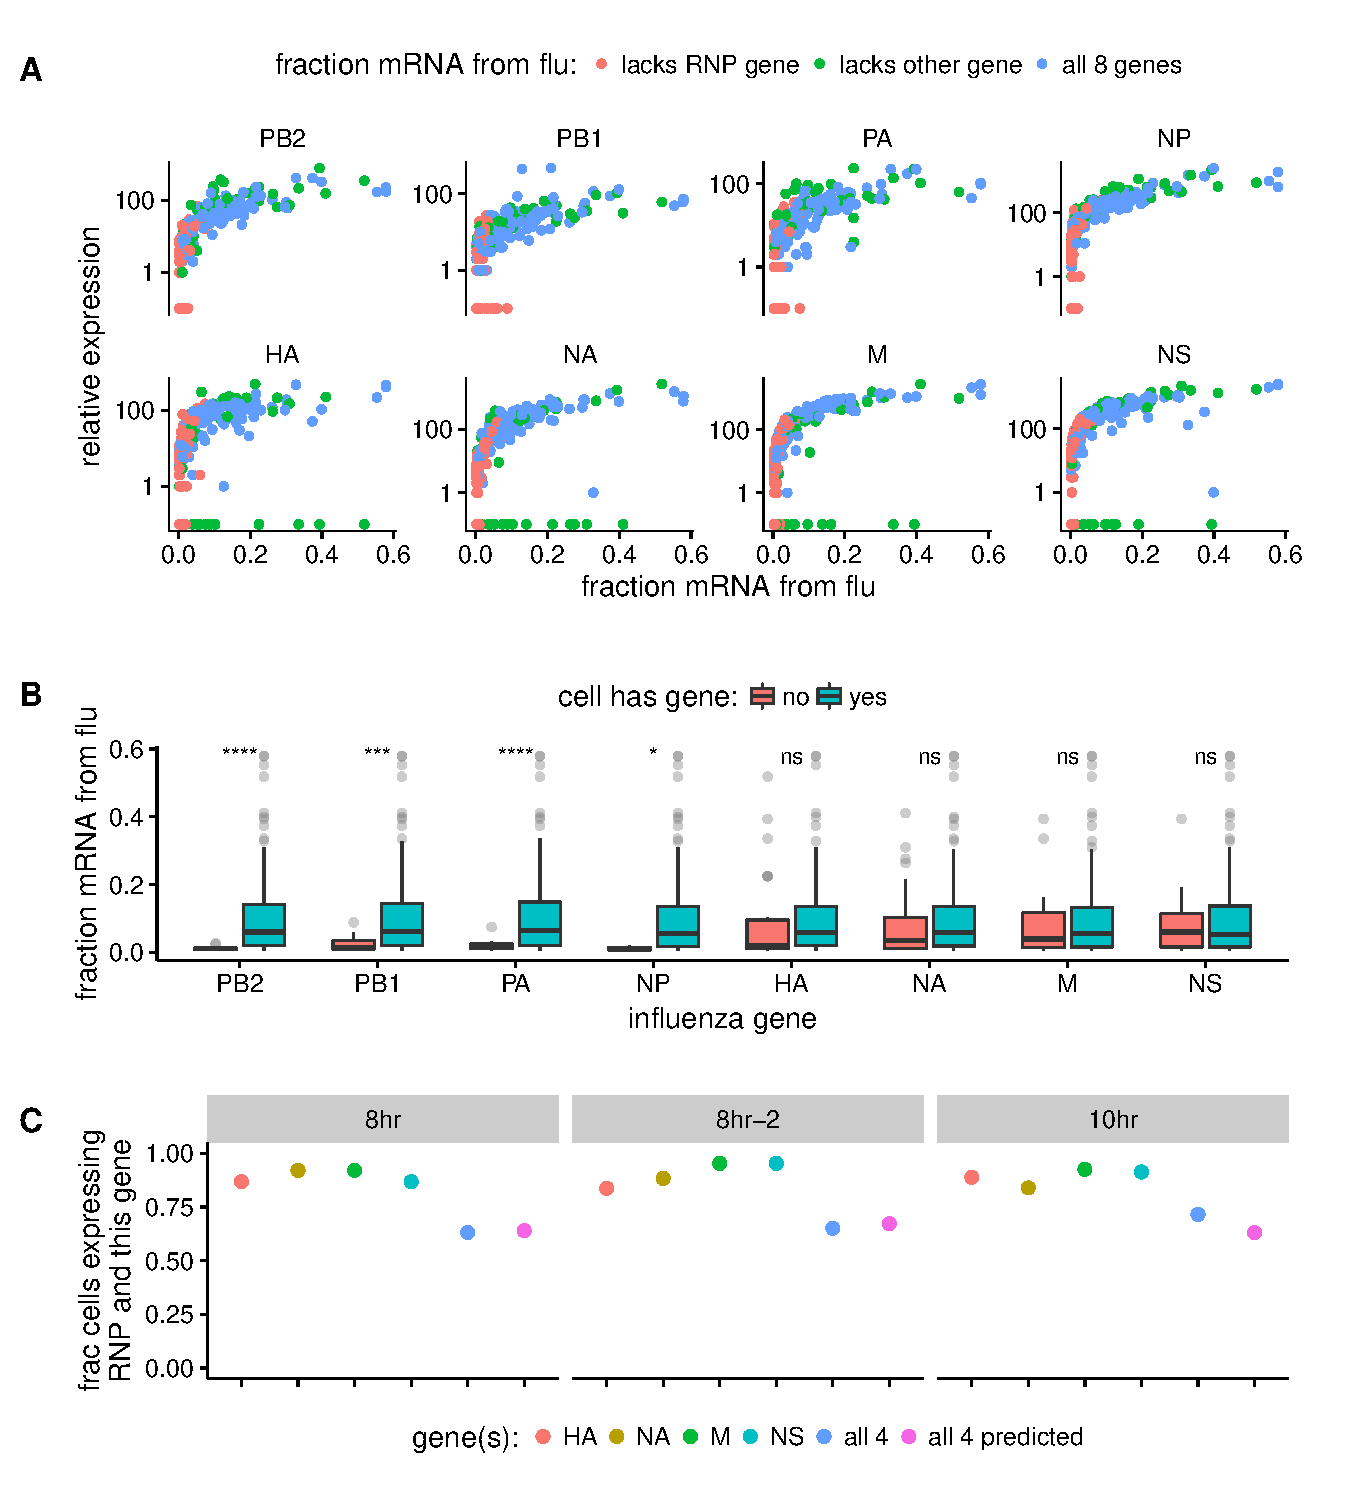
\includegraphics[width=\linewidth]{figures/p_flu_burden_flu_gene_merge.pdf}
\caption{\label{fig:fluburdenbyflugene}
The viral infection burden in individual cells as a function of the amount of each viral gene detected.
{\bf (A)} 
Fraction of mRNAs in each cell derived from virus as a function of the \emph{normalized} expression of each viral gene in that cell.
This plot shows that all cells with very high viral burden express all of the RNP genes, but some cells with high viral burden lack each of the other four viral genes.
{\bf (B)}
Statistical tests confirming that absence of viral RNP genes is significantly associated with reduced viral burden, but that the absence of the non-RNP genes does not lead to a clear decrease in viral burden.
}
\figsupp[Like panel (B) but for the 10-hr sample only.\label{figsupp:10hrfluburdenbyflugene}]{
The absence of viral RNP genes but \emph{not} non-RNP genes remains significantly associated with reduced viral burden when we examine only the 10-hr sample, which is the single timepoint with the most data points.
The difference for NP is no longer statistically significant due to low counts of infected cells lacking NP, but the qualitative trend remains.
}{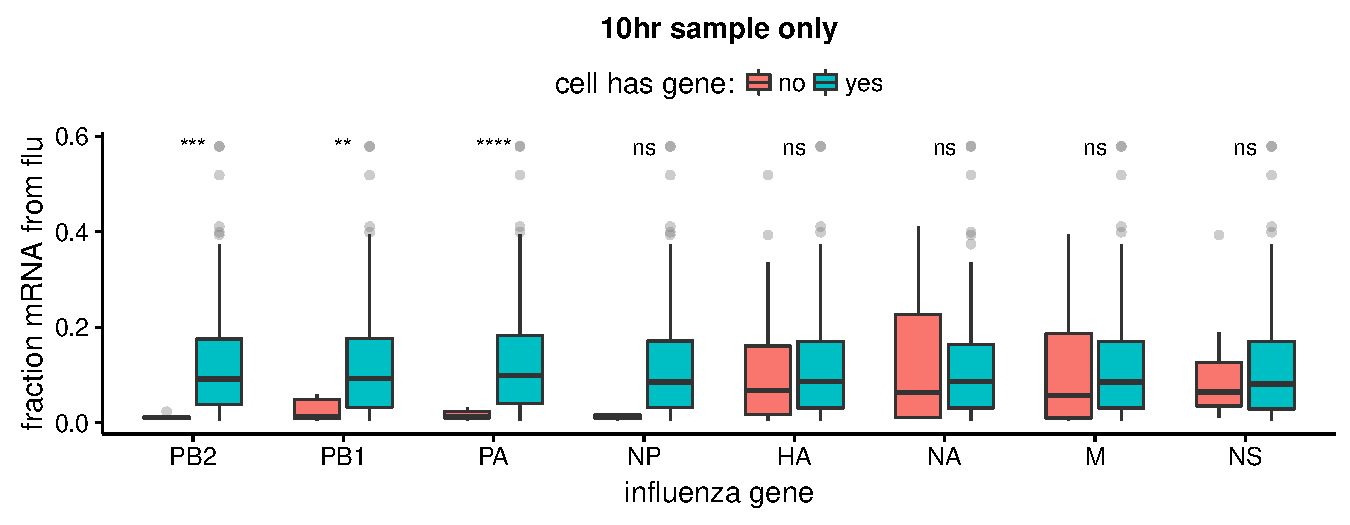
\includegraphics[width=\linewidth]{figures/p_10hr_flu_burden_flu_gene_test}}
\end{figure}

\subsection{Influenza Infections Are Predominated By Nonproductive Events.}
	We further wished to define metrics for presence/absence for a given segment and compare them to values obtained for other strains of influenza in order to understand the probability that a given infection could possibly produce infectious progeny. We decided to omit these calculations for PB1, PA, PB2, and NP. Using cyclohexamide treatment to limit cells to primary transcription alone, we find a 2-3 log reduction in mRNA levels of PB1 or HA relative to a 10h time point (supplemental figure). We therefore are not confident that our approach has the power to detect all semi-infectious events that result from a lack of polymerase or nucleoprotein segments. However, given the lack of effect absence of other segments appears to have on mRNA production, we proceeded to calculate the relative abundance of infectious events absent a given gene segment. 

\subsection{Influenza mRNA Ratios are Tightly Controlled}
	
	This and other reports have described the considerable heterogeneity produced as influenza infection progresses in tissue culture models. However, in stark contrast to our analyses above, the ratios of mRNAs generated by the eight segments appear to behave in a highly stereotyped fashion, with values roughly consistent with prior Northern Blot measurements of Influenza mRNA abundance. Staggeringly, this is true whether or not cells are expressing mRNAs from all eight segments, at all three time points,  and, in cells running the gamut of infectious burden --- although we must limit these conclusions to those cells engaging in secondary transcription given the caveats described above. Therefore while either noise in influenza replication or host variability can dramatically impact the amount of Influneza mRNA produced as a whole, these processes seem to, ignoring complete absence of a segment, act equally across the Influenza genome. This is consistent with more limited measurements showing positive correlations between several segments in vRNA measurements in single cells. It would therefore be inadvisable to search for the sources of the broad distribution in influenza replication in those steps that can impact segments independently of one-another, such as noise in the transition to cRNA or vRNA production, but rather only in those processes that could impact the kinetics of all segments equivalently, such as transport to the nucleus or availability of cellular resources. 


\subsection{Coinfection Occurs Early and Is Likely Adaptive For Influenza}
	While relatively rare in our dataset, those cells positively identified as containing both wild-type and synonymously barcoded influenza provide important insight into the nature of coinfection. It has been posited that coinfection can rescue nonproductive infections, potentially by providing missing genome equivalents. Brooke et al., for example observed increased co-occurrence of a given gene-segment pair as MOI was increased. When we examine our coinfected cells, we observe a much higher rate of expression of all eight segments (metric). Consistent with this model, we also observe that if we consider only one barcode or the other, that many of these infections would instead have been non-productive. Another observation that can be immediately procured is that, on the whole, coinfections have roughly balanced amounts of wild-type and barcoded segments. Others have noted that windows for coinfection are relatively narrow, and, these data directly suggest that this window is specifically narrow with respect to cRNA and vRNA production. If significant replication of viral genomes had already occurred, one would expect a much wider distribution of ratios than those observed. To support these observations, we used a virus in which the HA segment was replaced by GFP, allowing us to detect co-infection by this modified virus and wild-type WSN by flow cytometry. When we examine strictly co-infected cells, we observe that, as in our single-cell analysis, both HA and GFP are highly correlated --- indicating a tight window of coinfection --- and that a peak of low HA --- likely corresponding to primary transcription alone --- is greatly reduced. These data give credence to the sentiments of others that non-productive events are perhaps just productive events waiting to occur, and that the true dynamics underlying descriptions of ?MOI? are far more complex than we frequently give them credence and rely on assumptions that frequently prove incorrect. 




\begin{figure}
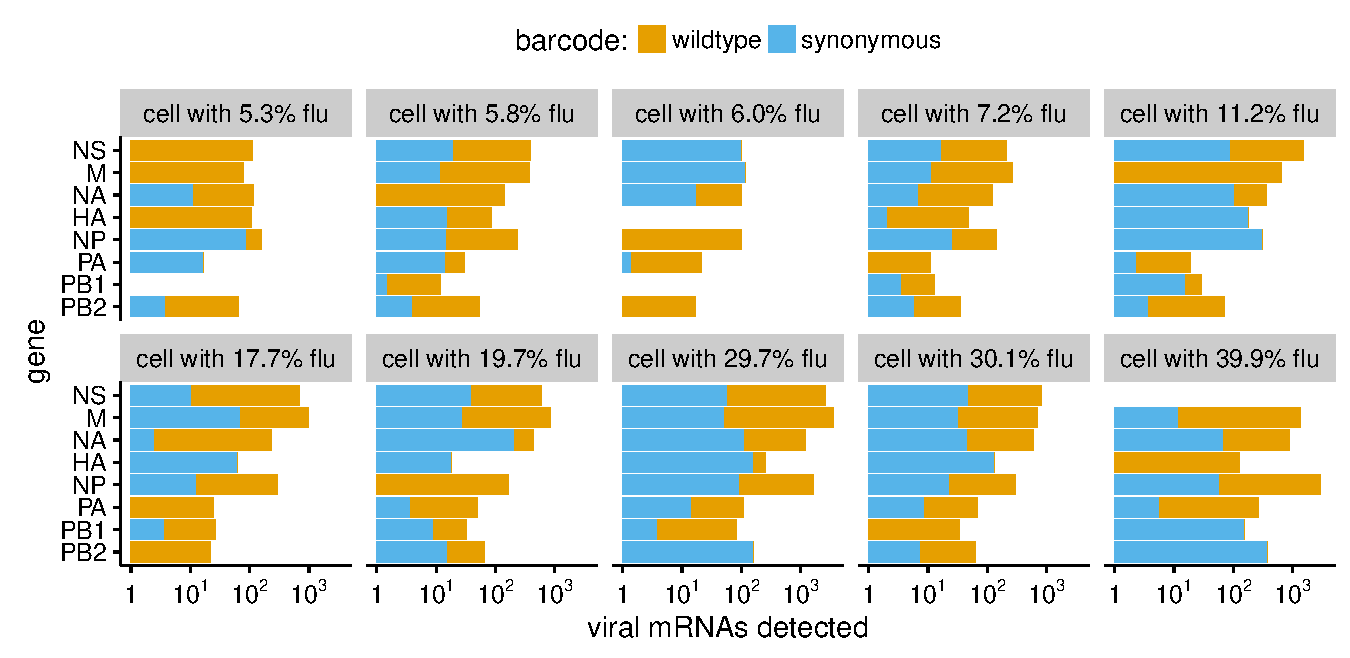
\includegraphics[width=\linewidth]{figures/p_coinfection.pdf}
\caption{\label{fig:coexpression}
Frequency of each viral gene segment in co-infected cells with at least 5\% of their mRNA derived from influenza.
The bars indicate the logarithm of the number of each viral mRNA detected, and the bars are colored in proportion to the fraction of those mRNAs that are derived from either wildtype or synonymous barcoded virus.
}
\figdata{The raw data plotted in this figure are in \texttt{p\_coinfection.csv}.}
\end{figure}

\subsection{Relative expression of different viral genes}
Figure~\ref{fig:fluexpr} shows some of this.
Cite \citet{hatada1989control} to show our relative expressions are consistent with that.
Maybe show a panel with just the 8-segment infections.

Maybe add a figure breaking this down among timepoints.

\begin{figure}
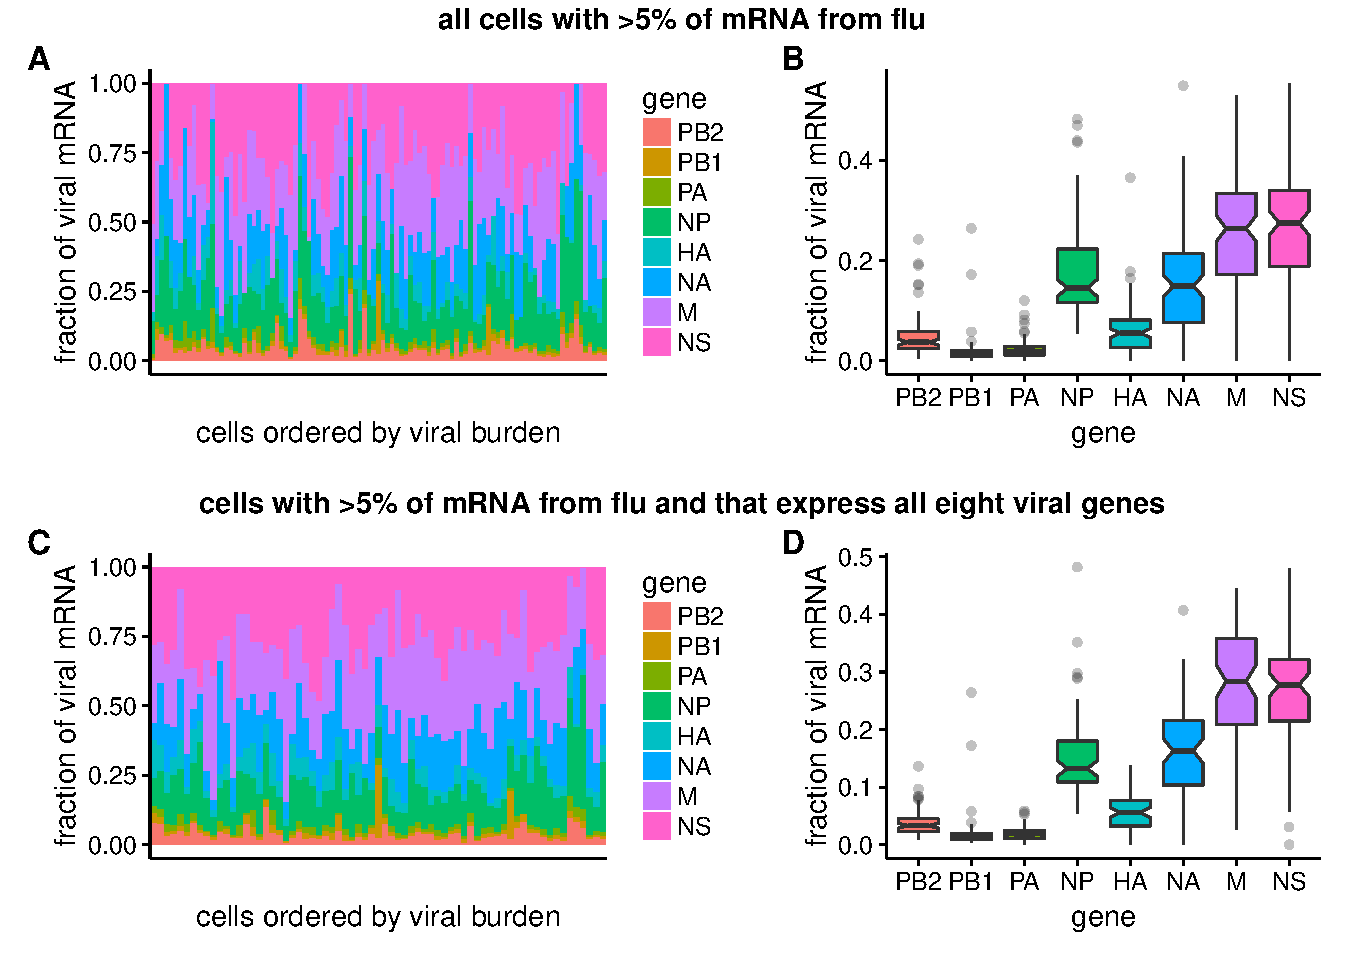
\includegraphics[width=\linewidth]{figures/p_flu_expr.pdf}
\caption{\label{fig:fluexpr}
Expression of individual influenza genes in highly infected cells (at least 5\% of total mRNA is viral).
{\bf (A)} 
The fraction of total mRNA from each influenza gene for each cell.
{\bf (B)}
Box plots showing the fraction of viral mRNA per cell that is derived from each influenza gene taken over all highly expressed cells.
The black line at the notch in each box is the median, and the top and bottom of the box indicate the first and third quartiles.
{\bf (C)}, {\bf (D)}
Like panels (A) and (B), but only show cells that express all eight viral genes.
}
\figdata{The raw data are in \texttt{p\_flu\_expr\_all.csv}.}
\end{figure}

\subsection{Host stuff}

\begin{figure}
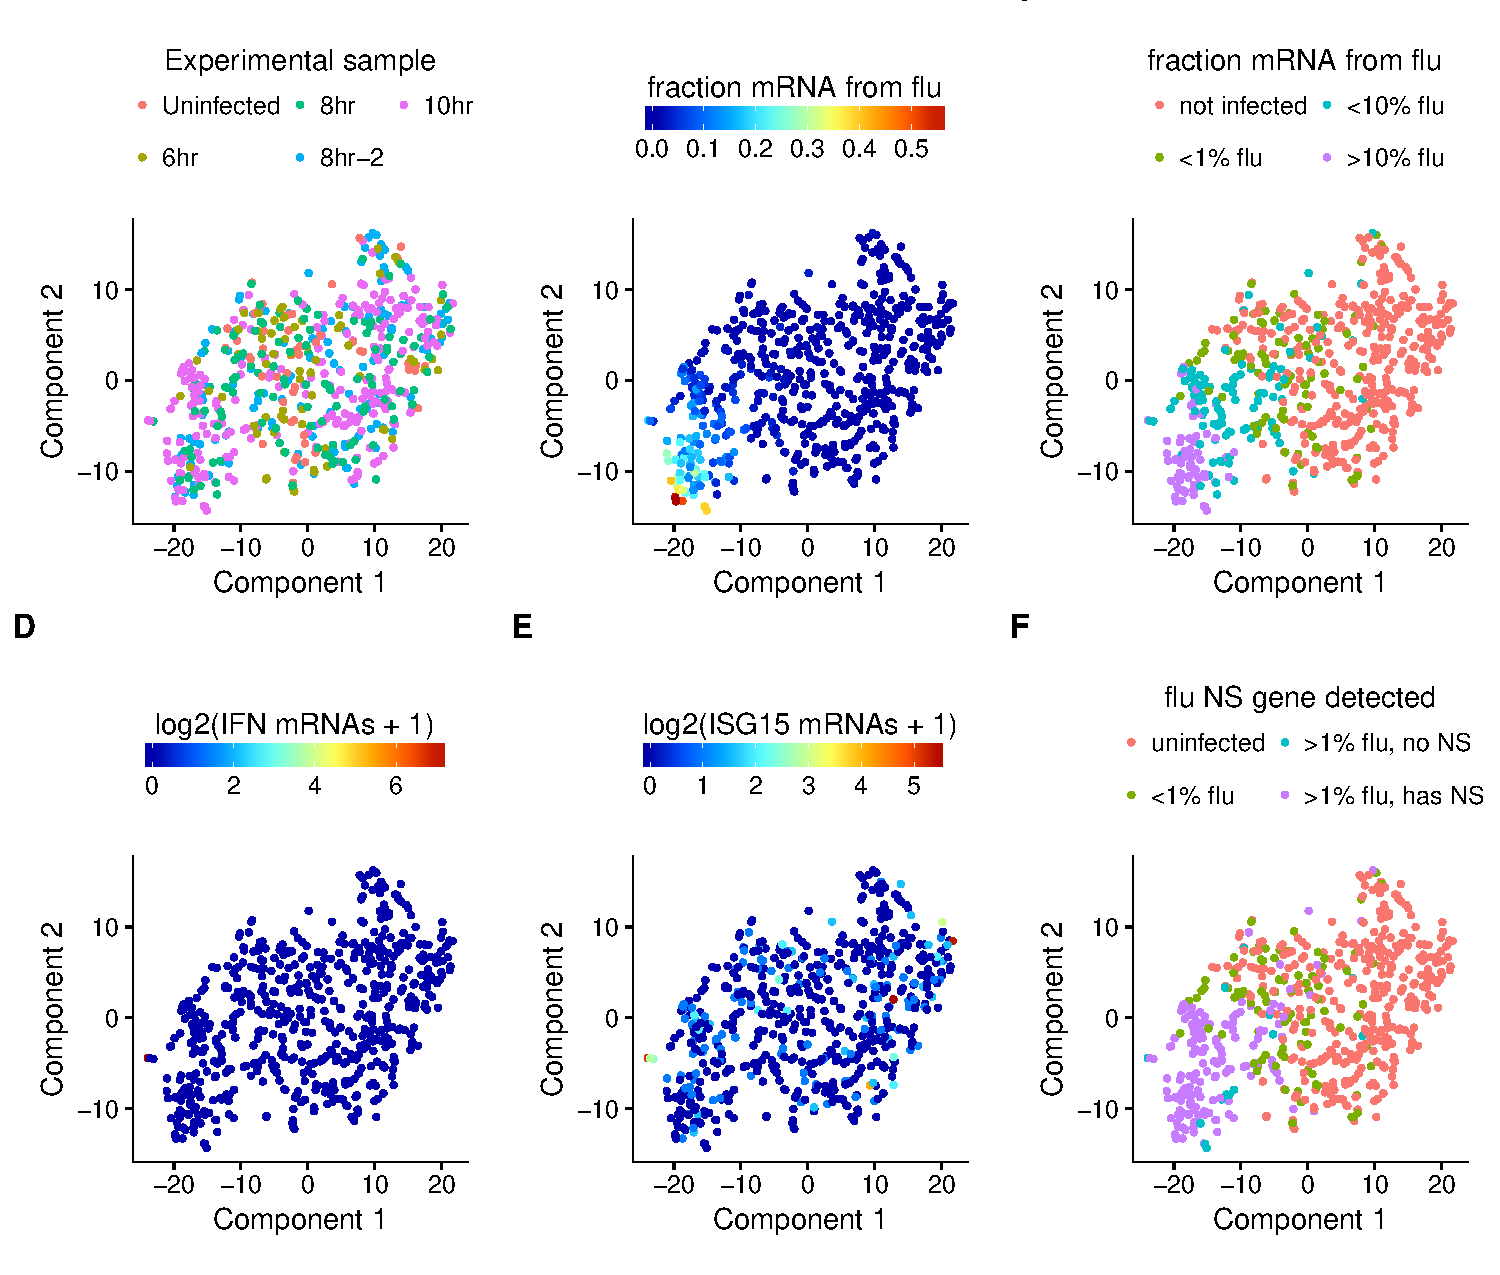
\includegraphics[width=\linewidth]{figures/p_small_tsne_merge.pdf}
\caption{\label{fig:tsne}
tSNE plots.
The layout is the same in all panels, but each panel colors the cells according to a different property.
{\bf (A), (B)}
Cells colored by the fraction of their mRNA that is viral.
{\bf (C)}
Cells colored by experimental sample.
While it is clear that cells from later timepoints often have more viral RNA, there are cells from earlier timepoints with a high viral burden and cells from late timepoints with a low viral burden.
{\bf (D)}
Cells colored by the number of type I and III interferon transcripts detected.
Only one cell has high expression of these interferons.
{\bf (E)}
Cells colored by the expression of the interferon-stimulate gene ISG15.
{\bf (F)}
For cells with at least 1\% of their reads from influenza, are the cells expressing the viral NS protein?
The one interferon-positive cell is lacking NS, but many other cells also lack NS but do not express interferon.
}
\end{figure}


\begin{figure}
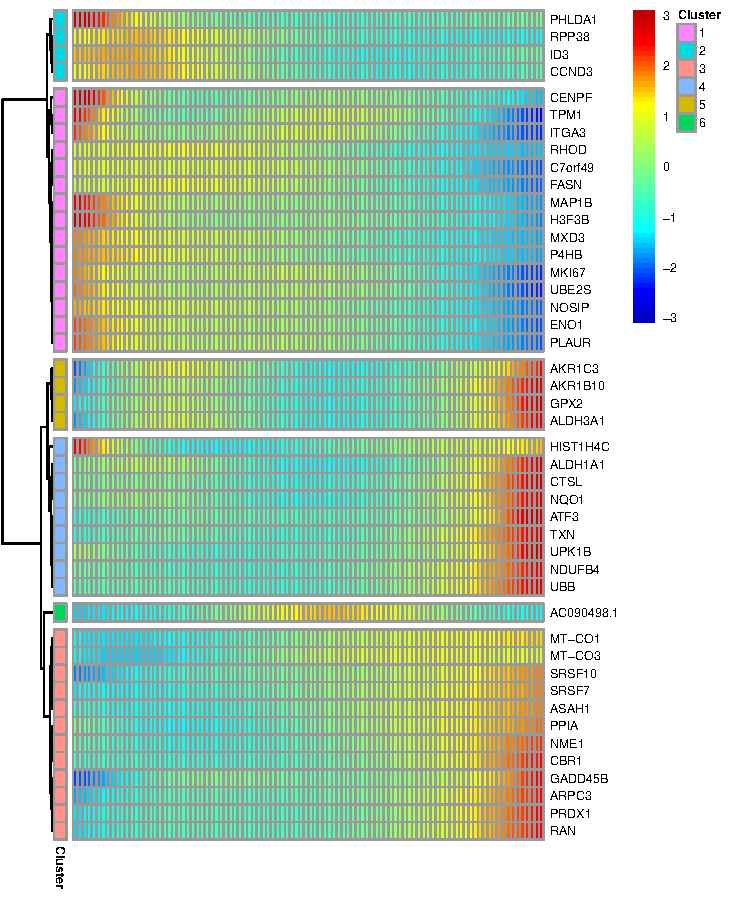
\includegraphics[width=0.8\linewidth]{figures/p_cellular_heatmap.pdf}
\caption{\label{fig:cellulargenes}
Cellular genes that are differentially expressed with respect to the amount of influenza mRNA in individual cells infected with full influenza virus containing all eight genes.
Shown are all genes differentially expressed with $Q < 0.1$.}
\figdata{The full results of the differential expression test is in \texttt{p\_sig\_cellular\_genes.csv}.}
\figdata{The results of a gene-set analysis are in \texttt{p\_sig\_cellular\_genes.csv}.}
\end{figure}

\section{Discussion}

\lipsum[9]

\section{Methods and Materials}

Guidelines can be included for standard research article sections, such as this one. 

\lipsum[3]

\section{Some \LaTeX{} Examples}
\label{sec:examples}

Use section and subsection commands to organize your document. 
\LaTeX{} handles all the formatting and numbering automatically. 
Use ref and label commands for cross-references.

\subsection{Figures and Tables}


If you use the following prefixes for your \verb|\label|:
%
\begin{description}
\item[Figures] \texttt{fig:}, e.g.~\verb|\label{fig:view}|
\item[Tables] \texttt{tab:}, e.g.~\verb|\label{tab:example}|
\item[Equations] \texttt{eq:}, e.g.~\verb|\label{eq:CLT}|
\item[Boxes] \texttt{box:}, e.g.~\verb|\label{box:simple}|
\end{description}
%
you can then use the convenience commands as in \verb|\FIG{cells}|, \ to generate cross-reference \FIG{view}. 

\subsection{Citations}

LaTeX formats citations and references automatically using the bibliography records in your .bib file, which you can edit via the project menu. 
Use the \verb|\cite| command for an inline citation, like \cite{trapnell2014pseudo}, and the \verb|\citep| command for a citation in parentheses \citep{trapnell2014pseudo}. 
The LaTeX template uses a slightly-modified Vancouver bibliography style. 
If your manuscript is accepted, the eLife production team will re-format the references into the final published form. 
\emph{It is not necessary to attempt to format the reference list yourself to mirror the final published form.}


\section{Acknowledgments}

Additional information can be given in the template, such as to not include funder information in the acknowledgments section.

\nocite{*} % This command displays all refs in the bib file
\bibliography{references}


\end{document}
